\documentclass[pdf]{beamer}
\mode<presentation>{}
%
\usecolortheme{orchid}
%

\usepackage[utf8]{inputenc}

\usepackage[sans]{dsfont}
\usepackage{amsmath}
\usepackage{gensymb}
\usepackage{mathtools}
\usepackage{eqparbox}

\newcommand{\op}[1]{\operatorname{#1}}
\newcommand{\bbf}[1]{\mathds{#1}}
\newcommand{\Z}{\bbf{Z}}
\newcommand{\R}{\bbf{R}}

\newtheorem*{satz*}{Satz}
\newtheorem*{cor*}{Korollar}
\newtheorem*{lemma*}{Lemma}
\newtheorem*{nb*}{N.B.}
\newtheorem*{def*}{Definition}
\newtheorem*{problem*}{Problem}
\newtheorem*{Aufgabe*}{Aufgabe}

\renewcommand*{\proofname}{Beweis}

\title{Bernsteinabbildungen, der $2$-Kozykel $\bbf{X}$, und der Raum der Orientierungen}
\author{Nicolas A. Schmidt}
\date{}

\begin{document}

%% title frame
\begin{frame}
   \titlepage
\end{frame}

\section{Einführung}
\begin{frame}{Überblick}
\begin{itemize}
   \item<2-> Zentrales Objekt: \textbf{Hecke-Algebren} \pause[3](Iwahori-Hecke-Algebren, affine Hecke-Algebren, pro-$p$-Iwahori Hecke-Algebren, \dots)
   \item<4->Genauer: \textbf{generische pro$\text{-}p$ Hecke-Algebren}
   \item<5-> Hecke Algebren $\mathcal{H}$ werden gebildet zu
      \begin{itemize}
         \item<6-> einer \textbf{Coxetergruppe}\pause[7] (bzw. einer ``pro-$p$ Coxetergruppe'')
         \item<8-> und einer \textbf{Familie von Parametern}
      \end{itemize}
   \item<9-> Zentrales Ziel: Bestimmung der Struktur von $\mathcal{H}$\pause[10], insbesondere Bestimmung des \textbf{Zentrums} $Z(\mathcal{H})$
      \pause[11]\[ Z(\mathcal{H}) = \{ z \in \mathcal{H}\ :\ zx = xz\text{ für alle } x \in \mathcal{H} \} \]
   \item<12-> Leitgedanke:
      \begin{itemize}
         \item<13-> Coxetergruppen sind \textit{geometrische} Objekte
         \item<14-> Verstehe $\mathcal{H}$ vermöge dieser Geometrie!
      \end{itemize}
\end{itemize}
\end{frame}

\begin{frame}{Das einfachste mathematische Objekt}
   \pause[3]
   \begin{tabular}[t]{rl}
      \textbf{Frage:}& Was ist die Gruppe der \textit{Symmetrien} von $\Delta$? \\
      \uncover<24->{\textbf{Antw.:}}& \pause[4]$W = \only<4-6>{\text{?}}\only<7-9>{\{ s, t, u, ... \}}\only<10>{\{ s, t, sts, ... \}}\only<11-13>{\{ s, t, sts, st, ... \}}\only<14-17>{\{ s, t, sts, st, \temporal<15>{\eqmakebox[BOX1][l]{$(st)^2$}}{\eqmakebox[BOX1][l]{$(st)^{-1}$}}{\eqmakebox[BOX1][l]{$ts$}}, \alt<-16>{\eqmakebox[BOX3][l]{$(st)^3$}}{\eqmakebox[BOX3][l]{$1$}}, ... \}}\only<18-22>{\eqmakebox[BOX2][l]{$\{ s, t, sts, st, ts, 1, ... \}$}}\only<23->{\eqmakebox[BOX2][l]{$\{ s, t, sts, st, ts, 1 \}$}}\only<22>{\eqmakebox[BOX4][r]{$\quad \subseteq\quad S_3$}}\only<23>{\eqmakebox[BOX4][r]{$ \quad =\quad S_3$}}$ \\
      \only<12-18,26-28>{\textbf{NB:}}\only<29-30>{\textbf{Wähle}}\only<31-32>{\textbf{Zu}}\only<33-36>{\textbf{Finde}}\only<46-53>{\textbf{NB:}}\only<54-65>{\textbf{Fazit:}} & \only<-18>{\uncover<12-18>{$st = \text{\textit{Drehung} um 120\degree} \pause[13]\quad\Rightarrow\quad \op{ord}(st) = 3$}}\only<26-28>{$W$ erhält $\mathfrak{H} = \{ s, t, u \}$\only<28->{ und \textit{Kammern}}}\only<29-30>{\textit{Fundamentalkammer}\only<30>{ $C$}}\only<31-32>{ $w \in W$\only<32>{ \textbf{betrachte} $wC$}}\only<33-36>{\textit{Gallerie}}\only<34-36>{ $(C, \uncover<35->{D}, \uncover<36->{E}, wC)$ }\only<46-48,50-53>{ $stswC = C$ }\only<48>{$\Rightarrow$ $wC = stsC$ }\only<49>{$\Rightarrow$ Jede Kammer hat die Form $sts\dots C$}\only<51-53>{ $\Rightarrow stsw = 1$ }\only<52-53>{$\Leftrightarrow$ $w = sts$}\only<53>{ $\Rightarrow W = \left<s,t\right>$}\only<54-56>{$W\only<54>{ = \left<s,t\right>}$ \only<55-56>{wirkt einfach transitiv auf Kammern}}\only<57>{$W = \text{Kammern}$}\only<58-63>{Ausdruck \only<58>{\eqmakebox[BOXeql][l]{$1$}}\only<59-61>{\eqmakebox[BOXeql][l]{$\uncover<59->{s}\uncover<60->{t}\uncover<61->{s}$}}\only<62-63>{\eqmakebox[BOXeql][l]{$tst$}} $\widehat{=}$ Gallerie $(1\only<59-61>{, s}\only<62-63>{, t}\only<60-61>{, st}\only<62-63>{, ts}\only<61>{, sts}\only<62-63>{, tst})$}\only<64-65>{$sts = tst$ \uncover<65>{\quad (``Zopfrelation'')}}
   \end{tabular}
   \pause[2]
   \begin{figure}
   \centering%
      \includegraphics<2-4>[width=0.5\textwidth]{graphics/triangle.eps}%
      \includegraphics<5>[width=0.5\textwidth]{graphics/triangle2.eps}%
      \includegraphics<6-7>[width=0.5\textwidth]{graphics/triangle3.eps}%
      \includegraphics<8>[width=0.5\textwidth]{graphics/triangle4.eps}%
      \includegraphics<9-19>[width=0.5\textwidth]{graphics/triangle5.eps}%
      \includegraphics<20>[width=0.5\textwidth]{graphics/triangle6.eps}%
      \includegraphics<21-23>[width=0.5\textwidth]{graphics/triangle7.eps}%
      \includegraphics<24>[width=0.5\textwidth]{graphics/triangle8.eps}%
      \includegraphics<25-26>[width=0.5\textwidth]{graphics/triangle9.eps}%
      \includegraphics<27-28>[width=0.5\textwidth]{graphics/triangle10.eps}%
      \includegraphics<29>[width=0.5\textwidth]{graphics/triangle11.eps}%
      \includegraphics<30-31>[width=0.5\textwidth]{graphics/triangle12.eps}%
      \includegraphics<32-34>[width=0.5\textwidth]{graphics/triangle13.eps}%
      \includegraphics<35>[width=0.5\textwidth]{graphics/triangle14.eps}%
      \includegraphics<36-37>[width=0.5\textwidth]{graphics/triangle15.eps}%
      \includegraphics<38>[width=0.5\textwidth]{graphics/triangle16.eps}%
      \includegraphics<39>[width=0.5\textwidth]{graphics/triangle17.eps}%
      \includegraphics<40>[width=0.5\textwidth]{graphics/triangle18.eps}%
      \includegraphics<41>[width=0.5\textwidth]{graphics/triangle19.eps}%
      \includegraphics<42>[width=0.5\textwidth]{graphics/triangle20.eps}%
      \includegraphics<43>[width=0.5\textwidth]{graphics/triangle21.eps}%
      \includegraphics<44>[width=0.5\textwidth]{graphics/triangle22.eps}%
      \includegraphics<45-46>[width=0.5\textwidth]{graphics/triangle23.eps}%
      \includegraphics<47-53,55>[width=0.5\textwidth]{graphics/triangle12.eps}%
      \includegraphics<54>[width=0.5\textwidth]{graphics/triangle31.eps}%
      \includegraphics<56>[width=0.5\textwidth]{graphics/triangle24.eps}%
      \includegraphics<57-58>[width=0.5\textwidth]{graphics/triangle25.eps}%
      \includegraphics<59>[width=0.5\textwidth]{graphics/triangle26.eps}%
      \includegraphics<60>[width=0.5\textwidth]{graphics/triangle27.eps}%
      \includegraphics<61>[width=0.5\textwidth]{graphics/triangle28.eps}%
      \includegraphics<62>[width=0.5\textwidth]{graphics/triangle29.eps}%
      \includegraphics<63-65>[width=0.5\textwidth]{graphics/triangle30.eps}%
   \end{figure}
\end{frame}

\begin{frame}{Zusammenfassung}
   \begin{itemize}
      \item<1-> $W$ $\widehat{=}$ $\text{Kammern}$\pause , $1$ $\widehat{=}$ $C$
      \item<3-> $W = \left<S\right>$
      \item<4-> $S = \text{Spiegelungen an den Hyperebenen die $C$ berühren}$
      \item<5-> $\mathfrak{H} = \text{Spiegelungen in $W$} \pause[6]= \{ wsw^{-1} : w \in W, s \in S \}$
      \item<7-> Ausdrücke $s_1 s_2 s_3 \dots$ $\widehat{=}$ Gallerien $(1, s_1, s_1s_2, s_1s_2s_3, \dots)$
   \end{itemize}
\end{frame}

\section{Grundbegriffe}
\begin{frame}{Coxetergruppen}
   \begin{definition}
      Eine \textit{Coxetergruppe} ist ein Paar $(W,S)$, so dass:
      \begin{itemize}
         \item<2-> $S$ besteht aus Elementen von $W$ der Ordnung $2$
         \item<3-> $W = \left<S\right>$
         \item<4-> $\ell(sw) < \ell(w) \Rightarrow w = ss_2 \dots s_r$ mit $r = \ell(w)$\quad\quad\quad (Bed. \text{E})
      \end{itemize}
      \pause[5]Hierbei ist
      \[ \ell(w) := \op{min} \{ r\ |\ w = s_1 \dots s_r\} \]
      die \textit{Länge} des Elementes $w$.
   \end{definition}
\begin{itemize}
   \item<6-> $\mathfrak{H} := \{ wsw^{-1} : w \in W, s \in S\}$
   \item<7-> $m(s,t) := \op{ord}(st)$\pause[8]\quad $\Rightarrow$\quad $\underbrace{sts\dots}_{m(s,t)} = \underbrace{tst\dots}_{m(s,t)}$
\end{itemize}
\end{frame}

\begin{frame}{Hecke-Algebren}
   \begin{itemize}
      \item<1-> $R$ - komm. Ring
      \item<2-> $(W,S)$ - Coxetergruppe
      \item<3-> $a_s, b_s \in R$ für $s \in S$; \pause[4] $s,t$ konjugiert in $W$ $\Rightarrow$ $a_s = a_t,\ b_s = b_t$
   \end{itemize}
   \pause[5]\begin{definition}
      Die \textit{Hecke-Algebra} $\mathcal{H}$ von $(W,S)$ \pause über $R$\pause , zu den Parametern $(a_s)_s$, $(b_s)_s$\pause , ist der $R$-Modul
      \[ \mathcal{H} := \bigoplus_{w \in W} R T_w \pause = \{ \sum_{w \in W} c_w T_w : c_w \in R,\enskip c_w = 0\enskip \text{für f.a. $w$}\} \]
      \pause versehen mit dem Produkt
      \begin{align*}
         T_w T_{w'} & = T_{ww'} && \text{falls $\ell(w)+\ell(w') = \ell(ww')$} \\
         \uncover<11->{T_s^2 & = a_s + b_s T_s && \text{($s \in S$)}}
      \end{align*}
   \end{definition}
\end{frame}

\begin{frame}{Das Leitbeispiel}
   Sei $a_s \equiv 1, b_s \equiv 0$: \pause $\Rightarrow T_s^2 = 1$
   \pause\begin{lemma}
      \begin{center}$T_w T_{w'} = T_{ww'} \quad \text{ für alle } w,w' \in W$\end{center}
   \end{lemma}
   \pause \begin{proof}
      \begin{itemize}
         \item<4-> O.B.d.A. $w = s$ und $\ell(sw') < \ell(w')$
         \item<5-> (Bed. E) $\Rightarrow$ $w' = s s_2 \ldots s_r$, $r = \ell(w')$
         \item<6-> $T_{w'} = T_{ss_2\ldots s_r} \pause[7] = T_s T_{s_2 \ldots s_r} \pause[8] = T_s T_v$
         \item<9-> $T_s T_{w'} = T_s T_s T_v \pause[10] = T_v \pause[11] = T_{sw'}$
      \end{itemize}
   \end{proof}
   \pause[12] $\Rightarrow \mathcal{H}$ ist nichts weiter als die Gruppenalgebra $R[W]$!
\end{frame}

\begin{frame}{Der Leitspruch}
   \begin{center}\LARGE Was für die Gruppenalgebra gilt, gilt auch für die Hecke-Algebra!\end{center}
\end{frame}

\begin{frame}{Das Zentrum von $R[W]$}
   \pause Sei $z = \sum_w c_w T_w \in Z(R[W])$.
   \begin{itemize}
      \item<3-> Für $g \in W$: $T_g z = z T_g \pause[4]\Rightarrow z = T_g z T_g^{-1}$
      \item<5-> $T_g z T_g^{-1} = \sum_w c_w T_{gwg^{-1}} \pause[6]= \sum_w c_{g^{-1}wg} T_w$
      \item<7-> $c_w = c_{g^{-1}wg}$ für alle $g \in W$
      \item<8-> d.h. $c_w$ hängt nur von $[w] = \{ g^{-1}wg : g \in G\}$ ab
      \item<9-> $\Rightarrow c_w = 0$ falls $[w]$ nicht endlich ist
   \end{itemize}
   \pause[10]Fazit:
   \begin{align*}Z(R[W]) & = \bigoplus_{[w] \text{ endl.}} R z_{[w]} \\
      \uncover<11->{z_{[w]} & := \sum_{w' \in [w]} T_{w'}}
   \end{align*}
\end{frame}

\begin{frame}{Affine Spiegelungsgruppen}
   \begin{itemize}
      \item<2-> Hatten betrachtet $W = D_3$\uncover<3->{ ($= S_3$)}
      \item<4-> Allg. $D_n = \text{(Symmetrien eines $n$-Ecks)}$\uncover<5->{ ($\neq S_n$ für $n > 3$)}
   \end{itemize}
   \begin{figure}
   \centering%
      \includegraphics<2-5>[width=0.5\textwidth]{graphics/triangle2.eps}%
      \includegraphics<6>[width=0.5\textwidth]{graphics/d4.eps}%
      \includegraphics<7>[width=0.5\textwidth]{graphics/d5.eps}%
      \includegraphics<8>[width=0.5\textwidth]{graphics/d6.eps}%
   \end{figure}
\end{frame}

\begin{frame}{Affine Spiegelungsgruppen}
   \begin{itemize}
      \item Gruppen $D_3$, $D_4$ sind besonders:\uncover<2->{ \textbf{kristallographisch}!}
      \item<6-> Genauer: \textit{Punktgruppen} kristallographischer Gruppen
      \item<7-> $G \leq \op{Isom}(\R^n)$ kristallograph. $\Leftrightarrow$ $G$ diskret und kokompakt
      \begin{itemize}
            \item<8->$\Leftrightarrow$ $G$ diskret und enthält volles Gitter (Satz v. Bieberbach)
      \item<9-> $G$ ist Erweiterung $1 \rightarrow X \rightarrow G \rightarrow W \rightarrow 1$
      \item<10-> $W$ Punktgruppe, $X$ Translationsgitter
      \item<11-> Spezialfall: $G = W\ltimes X$
   \end{itemize}
   \end{itemize}
   \begin{figure}
   \centering%
      \includegraphics<1>[height=5cm]{graphics/empty.eps}%
      \includegraphics<2>[height=5cm]{graphics/doppelspat.jpg}%
      \includegraphics<3>[height=5cm]{graphics/diverse.jpg}%
      \includegraphics<4>[height=5cm]{graphics/calcit.jpg}%
      \includegraphics<5-11>[height=5cm]{graphics/steinsalz.jpg}%
   \end{figure}
\end{frame}

\begin{frame}{Affine Spiegelungsgruppen}
   \begin{figure}
   \centering%
      \includegraphics<1>[width=.7\textwidth]{graphics/affcox1.eps}%
      \includegraphics<2>[height=.7\textwidth]{graphics/affcox2.eps}%
      \includegraphics<3>[height=.7\textwidth]{graphics/affcox3.eps}%
      \includegraphics<4>[height=.7\textwidth]{graphics/affcox4.eps}%
      \includegraphics<5>[height=.7\textwidth]{graphics/affcox5.eps}%
      \includegraphics<6>[height=.7\textwidth]{graphics/affcox-gone-wrong-pre.eps}%
      \includegraphics<7>[height=.7\textwidth]{graphics/affcox-gone-wrong.eps}%
      \includegraphics<8>[height=.7\textwidth]{graphics/affcox5.eps}%
      \includegraphics<9>[height=.7\textwidth]{graphics/affcox6.eps}%
      \includegraphics<10>[height=.7\textwidth]{graphics/affcox7.eps}%
      \includegraphics<11>[height=.7\textwidth]{graphics/affcox8.eps}%
   \end{figure}
\end{frame}

\begin{frame}{Affine Coxetergruppen}
   \begin{figure}
   \centering%
      \includegraphics<1>[height=.7\textwidth]{graphics/affcox9.eps}%
      \includegraphics<2>[height=.7\textwidth]{graphics/affcox10.eps}%
      \includegraphics<3>[height=.7\textwidth]{graphics/affcox9.eps}%
      \includegraphics<4>[height=.7\textwidth]{graphics/affcox11.eps}%
      \includegraphics<5>[height=.7\textwidth]{graphics/affcox12.eps}%
      \includegraphics<6>[height=.7\textwidth]{graphics/affcox13.eps}%
      \includegraphics<7>[height=.7\textwidth]{graphics/affcox14.eps}%
      \includegraphics<8>[height=.7\textwidth]{graphics/affcox15.eps}%
   \end{figure}
\end{frame}

\begin{frame}{$Z(R[W])$ für affine Coxetergruppen}
\begin{itemize}
   \item<2-> $W = W_0 \ltimes X$\quad -\quad $W_0$ endlich, $X$ Translationsgitter
   \item<3-> $R[X] \subseteq R[W]$\quad -\quad kommutative Unteralgebra
\end{itemize}

\pause[4]\begin{lemma*}
   Eine Konjugationsklasse in $W$ ist endlich genau dann wenn sie in $X$ enthalten ist.
\end{lemma*}
\begin{proof}<5->
   \begin{itemize}
      \item<5-> $w \in W_0$, $x \in X$: $x^{-1}wx = x^{-1}w(x) x$
      \item<6-> $\# \{ x^{-1}w(x) : x \in X\} = \infty$ falls $w \neq 1$
      \item<7-> Andererseits $[x] = \{ wxw^{-1}\ :\ w \in W \} = \{ wxw^{-1}\ :\ w \in W_0\}$ (endlich)
   \end{itemize}
\end{proof}
\end{frame}

\begin{frame}{$Z(R[W])$ für affine Coxetergruppen}
\begin{cor*}
   \begin{center}$Z(R[W]) = R[X]^{W_0}$\end{center}
\end{cor*}
\end{frame}

\begin{frame}{Eine Sackgasse (?)}
   \begin{align*} \uncover<2->{Z(R[W]) & = R[X]^{W_0} \\}
      \uncover<3->{Z(\mathcal{H}) & = \text{?}}
   \end{align*}
   \pause[4]\begin{problem*}
      Weder ist
   \[ X \longrightarrow \mathcal{H},\quad x \mapsto T_x \]
      ein (Monoid-)homomorphismus, noch ist
      \[ \bigoplus_{x \in X} RT_x \subseteq \mathcal{H} \]
      eine Unteralgebra, im allgemeinen.
   \end{problem*}
\end{frame}

\begin{frame}{Die Jagd nach den Bernsteinabbildungen}
   \pause[2]\begin{Aufgabe*} Zu jedem Ausdruck $s_1 \dots s_r$ wähle Vorzeichen $\varepsilon_1, \dots, \varepsilon_r \in \{ \pm \}$ derart, dass
   \[ T_{s_1}^{\varepsilon_1} \dots T_{s_r}^{\varepsilon_r} \in \mathcal{H} \]
   nur von dem Element $w = s_1 \dots s_r \in W$ abhängt.
\end{Aufgabe*}
\pause[3]\begin{center}\begin{tabular}{rcl}
      Ausdrücke $s_1 \dots s_r$ & $\widehat{=}$ &Gallerien \\ & & \\
      \uncover<4->{Ausdrücke $T_{s_1}^{\varepsilon_1} \dots T_{s_r}^{\varepsilon_r}$ & $\widehat{=}$ & \uncover<5->{\textit{gefärbte} Gallerien}}
\end{tabular}\end{center}
\end{frame}

\begin{frame}{Die Jagd nach den Bernsteinabbildungen}
   \begin{columns}
      \begin{column}{.381966\textwidth}
         \begin{tabular}{rl}Ausdruck: & %
         \only<1>{$ $}%
         \only<2>{$s_1$}%
         \only<3>{$s_2$}%
         \only<4>{$s_0$}%
         \only<5>{$s_1$}%
         \only<6>{$s_1 s_2$}%
         \only<7>{$s_1 s_2 s_1$}%
         \only<8>{$T_{s_1} T_{s_2} T_{s_1}$}%
         \only<9>{$T_{s_1}^{-1} T_{s_2} T_{s_1}$}%
         \only<10>{$T_{s_1}^{-1} T_{s_2}^{-1} T_{s_1}$}%
         \only<11>{$T_{s_1}^{-1} T_{s_2}^{-1} T_{s_1}^{-1}$}%
         \end{tabular}
      \end{column}
      \begin{column}{.618034\textwidth}
         \begin{figure}
            \centering%
            \includegraphics<1>[width=\textwidth]{graphics/uncolgal.eps}%
            \includegraphics<2>[width=\textwidth]{graphics/uncolgal2.eps}%
            \includegraphics<3>[width=\textwidth]{graphics/uncolgal3.eps}%
            \includegraphics<4>[width=\textwidth]{graphics/uncolgal4.eps}%
            \includegraphics<5>[width=\textwidth]{graphics/uncolgal2.eps}%
            \includegraphics<6>[width=\textwidth]{graphics/uncolgal5.eps}%
            \includegraphics<7>[width=\textwidth]{graphics/uncolgal6.eps}%
            \includegraphics<8>[width=\textwidth]{graphics/colgal1.eps}%
            \includegraphics<9>[width=\textwidth]{graphics/colgal2.eps}%
            \includegraphics<10>[width=\textwidth]{graphics/colgal3.eps}%
            \includegraphics<11>[width=\textwidth]{graphics/colgal4.eps}%
         \end{figure}
      \end{column}
   \end{columns}
\end{frame}

\begin{frame}{Die Jagd nach den Bernsteinabbildungen}
   \only<1>{\begin{Aufgabe*} Zu jedem \textbf{Ausdruck} $s_1 \dots s_r$ wähle \textbf{Vorzeichen} $\varepsilon_1, \dots, \varepsilon_r \in \{ \pm \}$ derart, dass
   \[ T_{s_1}^{\varepsilon_1} \dots T_{s_r}^{\varepsilon_r} \in \mathcal{H} \]
   nur von dem \textbf{Element} $w = s_1 \dots s_r \in W$ abhängt.
\end{Aufgabe*}}%
\only<2>{\begin{Aufgabe*} Zu jeder \textbf{Gallerie} wähle eine \textbf{Färbung} derart, dass das zugehörige Element
   \[ T_{s_1}^{\varepsilon_1} \dots T_{s_r}^{\varepsilon_r} \in \mathcal{H} \]
   nur vom \textbf{Endpunkt} der Gallerie abhängt.
\end{Aufgabe*}}
\end{frame}

\begin{frame}{Die Jagd nach den Bernsteinabbildungen}
   \begin{columns}
      \begin{column}{.45\textwidth}
         \begin{tabular}{rl}Ausdruck: & %
            \only<1>{$T_{s_1} T_{s_2} T_{s_1}$}%
            \only<2>{$T_{s_1} T_{s_2} T_{s_1} T_{s_2}^{-1}$}%
            \only<3>{$T_{s_1} T_{s_2} T_{s_1} T_{s_2}^{-1} T_{s_1}^{-1}$}%
            \only<4-5>{$T_{s_1} T_{s_2} T_{s_1} T_{s_2}^{-1} T_{s_1}^{-1} T_{s_2}^{-1}$}%
            \only<6>{$T_{s_1} T_{s_2} T_{s_1} T_{s_2}^{-1} T_{s_1}^{-1}$}%
            \only<7>{$T_{s_1} T_{s_2} T_{s_1} T_{s_2}^{-1}$}%
            \only<8>{$T_{s_1} T_{s_2} T_{s_1}$}%
            \only<9>{$T_{s_1}^{-1} T_{s_2} T_{s_1}$}%
            \only<10>{$T_{s_1}^{-1} T_{s_2}^{-1} T_{s_1}$}%
            \only<11>{$T_{s_1}^{-1} T_{s_2}^{-1} T_{s_1}^{-1}$}%
            \only<12>{$T_{s_1} T_{s_2}^{-1} T_{s_1}^{-1}$}%
            \only<13>{$T_{s_1} T_{s_2} T_{s_1}^{-1}$}%
            \only<14>{$T_{s_1} T_{s_2} T_{s_1}$}%
            \only<15>{$T_{s_0} T_{s_0}^{-1}$}%
         \end{tabular} \\
         \begin{figure}
            \centering%
            \includegraphics<1>[width=\textwidth]{graphics/colgal5l.eps}%
            \includegraphics<2>[width=\textwidth]{graphics/colgal6l.eps}%
            \includegraphics<3>[width=\textwidth]{graphics/colgal7l.eps}%
            \includegraphics<4>[width=\textwidth]{graphics/colgal8l.eps}%
            \includegraphics<5>[width=\textwidth]{graphics/colgal9l.eps}%
            \includegraphics<6>[width=\textwidth]{graphics/colgal10l.eps}%
            \includegraphics<7>[width=\textwidth]{graphics/colgal11l.eps}%
            \includegraphics<8>[width=\textwidth]{graphics/colgal12l.eps}%
            \includegraphics<9>[width=\textwidth]{graphics/colgal13l.eps}%
            \includegraphics<10>[width=\textwidth]{graphics/colgal14l.eps}%
            \includegraphics<11>[width=\textwidth]{graphics/colgal15l.eps}%
            \includegraphics<12>[width=\textwidth]{graphics/colgal16l.eps}%
            \includegraphics<13>[width=\textwidth]{graphics/colgal17l.eps}%
            \includegraphics<14>[width=\textwidth]{graphics/colgal12l.eps}%
            \includegraphics<15>[width=\textwidth]{graphics/colgal18l.eps}%
         \end{figure}
      \end{column}
      \begin{column}[c]{.1\textwidth}
      \begin{center}$=$\end{center}
      \end{column}
      \begin{column}{.45\textwidth}
         \begin{tabular}{rl}Ausdruck: & %
         \only<1>{$T_{s_2} T_{s_1} T_{s_2}$}%
         \only<2>{$T_{s_2} T_{s_1}$}%
         \only<3>{$T_{s_2}$}%
         \only<4-5>{$ $}%
         \only<6>{$T_{s_2}$}%
         \only<7>{$T_{s_2} T_{s_1}$}%
         \only<8>{$T_{s_2} T_{s_1} T_{s_2}$}%
         \only<9>{$T_{s_2} T_{s_1} T_{s_2}^{-1}$}%
         \only<10>{$T_{s_2} T_{s_1}^{-1} T_{s_2}^{-1}$}%
         \only<11>{$T_{s_2}^{-1} T_{s_1}^{-1} T_{s_2}^{-1}$}%
         \only<12>{$T_{s_2}^{-1} T_{s_1}^{-1} T_{s_2}$}%
         \only<13>{$T_{s_2}^{-1} T_{s_1} T_{s_2}$}%
         \only<14>{$T_{s_2} T_{s_1} T_{s_2}$}%
         \only<15>{$ $}%
         \end{tabular} \\
         \begin{figure}
            \centering%
            \includegraphics<1>[width=\textwidth]{graphics/colgal5r.eps}%
            \includegraphics<2>[width=\textwidth]{graphics/colgal6r.eps}%
            \includegraphics<3>[width=\textwidth]{graphics/colgal7r.eps}%
            \includegraphics<4>[width=\textwidth]{graphics/colgal8r.eps}%
            \includegraphics<5>[width=\textwidth]{graphics/colgal9r.eps}%
            \includegraphics<6>[width=\textwidth]{graphics/colgal10r.eps}%
            \includegraphics<7>[width=\textwidth]{graphics/colgal11r.eps}%
            \includegraphics<8>[width=\textwidth]{graphics/colgal12r.eps}%
            \includegraphics<9>[width=\textwidth]{graphics/colgal13r.eps}%
            \includegraphics<10>[width=\textwidth]{graphics/colgal14r.eps}%
            \includegraphics<11>[width=\textwidth]{graphics/colgal15r.eps}%
            \includegraphics<12>[width=\textwidth]{graphics/colgal16r.eps}%
            \includegraphics<13>[width=\textwidth]{graphics/colgal17r.eps}%
            \includegraphics<14>[width=\textwidth]{graphics/colgal12r.eps}%
            \includegraphics<15>[width=\textwidth]{graphics/colgal18r.eps}%
         \end{figure}
      \end{column}
   \end{columns}
\end{frame}

\begin{frame}{Orientierungen von Coxetergruppen}
   \begin{def*}
      Eine \textit{Orientierung} einer Coxetergruppe $(W,S)$ ist eine Abbildung $\mathfrak{o}: W\times S \rightarrow \{\pm 1\}$ derart, dass\\[8pt]
      \pause[2]\begin{tabular}{rl}
         (OR1) & $\mathfrak{o}(ws,s) = -\mathfrak{o}(w,s)$ \\[10pt]
         \pause[3](OR2) & $(\mathfrak{o}(w, s), \mathfrak{o}(ws, t), \mathfrak{o}(wst, s), \mathfrak{o}(wsts, s), \dots)$ \pause[4] und \\[3pt]
         & $(\mathfrak{o}(w, t), \mathfrak{o}(wt, s), \mathfrak{o}(wts, t), \mathfrak{o}(wtst, s), \dots)$ \\[3pt]
         \pause[5] & haben (resp.) die Gestalt \\[5pt]
         & $(\underbrace{+, \dots, +}_k, \underbrace{-, \dots, -}_{m(s,t)-k})$ und $(\underbrace{-, \dots, -}_{m(s,t)}, \underbrace{+, \dots, +}_k)$ \\[20pt]
         & \pause[6] oder umgekehrt\pause[7], falls $m(s,t) < \infty$.
      \end{tabular}
   \end{def*}
\end{frame}

\begin{frame}{Die Bernsteinabbildung $\theta$}
   \uncover<5->{Sei $a_s \in R^\times$ für alle $s$. Dann gilt}
   \begin{satz*}
      Zu jeder Orientierung $\mathfrak{o}$ gibt es genau eine Abbildung
      \[ \theta_\mathfrak{o}: W \longrightarrow \mathcal{H}^\times \]
      derart, dass\pause[2]
      \[ \theta_\mathfrak{o}(w) = T_{s_1}^{\varepsilon_1} \dots T_{s_r}^{\varepsilon_r} \]
      \pause[3]für jeden Ausdruck $w = s_1 \dots s_r$, \pause[4] wobei $\varepsilon_i = \mathfrak{o}(s_1 \dots s_{i-1}, s_i)$.
   \end{satz*}
   \pause[6]\begin{lemma*}
      Für jedes $w \in W$ ist $T_w$ eine Einheit, und für $s \in S$ ist
      \[ T_s^{-1} = a_s^{-1}(T_s - b_s) \]
   \end{lemma*}
\end{frame}

\begin{frame}{Die Menge der Orientierungen}
   \begin{def*}
      \begin{center}$\mathcal{O}(W,S) := \{ \mathfrak{o} \in \{\pm 1\}^{W\times S}\ :\ \text{$\mathfrak{o}$ ist Orientierung}\}$\end{center}
   \end{def*}
\end{frame}

\begin{frame}{Die Menge der Orientierungen}
   \begin{lemma*}
      Auf $\mathcal{O}(W,S)$ wirkt $W$ rechts derart, dass
      \[ (\mathfrak{o}\bullet w)(w',s) = \mathfrak{o}(ww',s) \]
      \pause[2]Ferner ist dort eine Involution $\mathfrak{o} \mapsto \mathfrak{o}^{\op{op}}$ durch
      \[ \mathfrak{o}^{\op{op}}(w,s) = -\mathfrak{o}(w,s) \]
      gegeben, welche mit der Rechtswirkung kommutiert.
   \end{lemma*}
\end{frame}

\begin{frame}{Die Produktformel}
   \begin{lemma*}
      \begin{center}$\theta_{\mathfrak{o}}(w) \theta_{\mathfrak{o}\bullet w}(w') = \theta_{\mathfrak{o}}(ww')$\end{center}
   \end{lemma*}
   \pause[2] 
   \begin{cor*}
      \[ \op{Stab}_W(\mathfrak{o}) \longrightarrow \mathcal{H}^\times,\quad w \mapsto \theta_\mathfrak{o}(w) \]
      ist ein Gruppenhomomorphismus.
   \end{cor*}
   \pause[3]$\Rightarrow$ Finde Orientierung $\mathfrak{o}$ welche invariant unter $X \leq W$ ist!
\end{frame}

\begin{frame}{Kammerorientierungen}
   \pause[2]\begin{lemma*}
      Für jedes $w_0 \in W$ definiert
      \[ \mathfrak{o}_{w_0}(w,s) := \begin{cases} +1 &\text{ falls $\ell(w_0^{-1}ws) < \ell(w_0^{-1}w)$} \\
         -1 &\text{ falls $\ell(w_0^{-1}ws) > \ell(w_0^{-1}w)$} \end{cases} \]
      eine Orientierung, die \textit{Kammerorientierung zu $w_0$ hin}.
   \end{lemma*}
\end{frame}

\begin{frame}{Kammerorientierungen}
   \begin{proof}
      \begin{figure}
         \centering%
         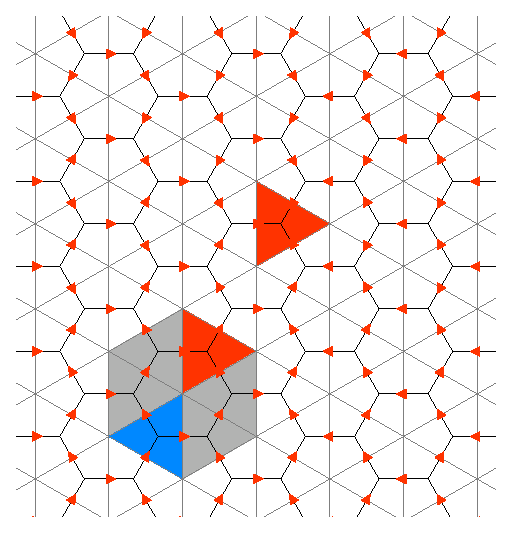
\includegraphics[width=.5\textwidth]{graphics/orientations-and-cayley-graph.eps}%
      \end{figure}
   \end{proof}
\end{frame}

\begin{frame}{Die Menge der Orientierungen im endlichen Fall}
   Sei $W$ endlich.
   \pause\begin{satz*}
      \begin{center}$W \longrightarrow \mathcal{O}(W,S),\quad w \mapsto \mathfrak{o}_{w}$\end{center}
      ist bijektiv.
   \end{satz*}
   \pause\begin{nb*}
      \begin{center}$\mathfrak{o}_{w}^{\op{op}} = \mathfrak{o}_{w_0 w}$\end{center}
      wobei $w_0 \in W$ das längste Element ist.
   \end{nb*}
\end{frame}

\begin{frame}{Der \textit{Raum} der Orientierungen}
   \begin{itemize}
      \item<2-> $\{ \pm 1\}^{W \times S}$ ist ein kompakter top. Raum (Satz v. Tychonoff)
   \end{itemize}
   \pause[3]\begin{lemma*}
      Die Teilmenge
      \[ \mathcal{O}(W,S)\enskip \subseteq\enskip \{ \pm 1 \}^{W \times S} \]
      ist \textit{abgeschlossen}.
   \end{lemma*}
   \pause \begin{lemma*}
      Die Teilmenge
      \begin{center}$\mathcal{O}_{\text{Kammer}} := \{ \mathfrak{o}_w, \mathfrak{o}_w^{\op{op}}\ :\ w \in W\}\enskip \subseteq\enskip \mathcal{O}(W,S)$\end{center}
      ist \textit{diskret}, wenn $\# S < \infty$.
   \end{lemma*}
\end{frame}

\begin{frame}{Randorientierungen}
   \begin{def*}
      \begin{center}$\mathcal{O}_{\text{Rand}} := \partial \mathcal{O}_{\op{Kammer}}$\end{center}
   \end{def*}
   \pause\begin{cor*}
      \begin{center}$\mathcal{O}_{\text{Rand}} \neq \emptyset$\end{center}
      falls $\# W = \infty$ und $\# S < \infty$.
   \end{cor*}
\end{frame}

\begin{frame}{Die hyperbolische Coxetergruppe $\op{PGL}_2(\Z)$}
   \begin{figure}
      \centering%
      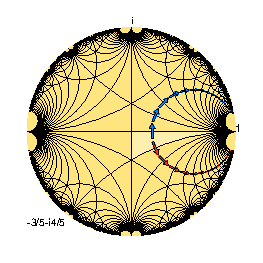
\includegraphics[width=.8\textwidth]{graphics/hyperbolic-orientation.eps}%
   \end{figure}
\end{frame}

\begin{frame}{Sphärische Orientierungen}
   $W = W_0 \ltimes X$ - affine Coxetergruppe
   \begin{columns}
      \begin{column}{.381966\textwidth}
         \begin{itemize}
            \item<2-> Weylkammer $V$
            \item<9-> $\Phi^+_V = \{ \alpha : V \subseteq \alpha \}$
            \item<13-> $H \in \mathfrak{H}$: \uncover<14->{$U_H$}\uncover<17->{ positiv falls parallel zu $\alpha \in \Phi^+_V$}
            \item<22-> $\mathfrak{o}_V(w,s) := \begin{cases} +1 : ws \in U^+_H \\ -1 : ws \in U^-_H\end{cases}$ \uncover<23->{wobei $H = wsw^{-1}$}
            \item<25-> $X \subseteq \op{Stab}(\mathfrak{o}_V)$
            \item<26-> $\mathfrak{o}_V \in \mathcal{O}_{\text{Rand}}$
            \item<28-> $\mathfrak{o}_V = \lim_n \mathfrak{o}_{w_n}$
         \end{itemize}
      \end{column}
      \begin{column}{.618034\textwidth}
         \begin{figure}
            \centering%
            \includegraphics<1>[width=\textwidth]{graphics/sphor1.eps}%
            \includegraphics<2>[width=\textwidth]{graphics/sphor2.eps}%
            \includegraphics<3>[width=\textwidth]{graphics/sphor3.eps}%
            \includegraphics<4>[width=\textwidth]{graphics/sphor4.eps}%
            \includegraphics<5>[width=\textwidth]{graphics/sphor5.eps}%
            \includegraphics<6>[width=\textwidth]{graphics/sphor6.eps}%
            \includegraphics<7>[width=\textwidth]{graphics/sphor7.eps}%
            \includegraphics<8-9>[width=\textwidth]{graphics/sphor2.eps}%
            \includegraphics<10>[width=\textwidth]{graphics/sphor8.eps}%
            \includegraphics<11>[width=\textwidth]{graphics/sphor10.eps}%
            \includegraphics<12>[width=\textwidth]{graphics/sphor9.eps}%
            \includegraphics<13>[width=\textwidth]{graphics/sphor11.eps}%
            \includegraphics<14>[width=\textwidth]{graphics/sphor12.eps}%
            \includegraphics<15>[width=\textwidth]{graphics/sphor13.eps}%
            \includegraphics<16-17>[width=\textwidth]{graphics/sphor11.eps}%
            \includegraphics<18>[width=\textwidth]{graphics/sphor14.eps}%
            \includegraphics<19>[width=\textwidth]{graphics/sphor15.eps}%
            \includegraphics<20>[width=\textwidth]{graphics/sphor16.eps}%
            \includegraphics<21-23>[width=\textwidth]{graphics/sphor11.eps}%
            \includegraphics<24-26>[width=\textwidth]{graphics/sphor17.eps}%
            \includegraphics<27-28>[width=\textwidth]{graphics/sphor18.eps}%
            \includegraphics<29>[width=\textwidth]{graphics/sphor19.eps}%
         \end{figure}
      \end{column}
   \end{columns}
\end{frame}
\end{document}
